\documentclass[11pt,a4paper]{article}

% --- Packages ---
\usepackage[utf8]{inputenc}
\usepackage{geometry}
\geometry{margin=1in}
\usepackage{amsmath, amssymb}
\usepackage{graphicx}
\usepackage{hyperref}
\usepackage{booktabs}
\usepackage{listings}
\usepackage{xcolor}
\usepackage{cite}
\usepackage{caption}
\usepackage{float}

% --- Code Listing Style ---
\definecolor{codegreen}{rgb}{0,0.6,0}
\definecolor{codegray}{rgb}{0.5,0.5,0.5}
\definecolor{codepurple}{rgb}{0.58,0,0.82}
\definecolor{backcolour}{rgb}{0.95,0.95,0.92}

\lstdefinestyle{mystyle}{
    backgroundcolor=\color{backcolour},   
    commentstyle=\color{codegreen},
    keywordstyle=\color{magenta},
    numberstyle=\tiny\color{codegray},
    stringstyle=\color{codepurple},
    basicstyle=\ttfamily\footnotesize,
    breakatwhitespace=false,         
    breaklines=true,                 
    captionpos=b,                    
    keepspaces=true,                 
    numbers=left,                    
    numbersep=5pt,                  
    showspaces=false,                
    showstringspaces=false,
    showtabs=false,                  
    tabsize=2
}
\lstset{style=mystyle}

% --- Custom JSON Definition for Listings ---
\lstdefinelanguage{json}{
    basicstyle=\normalfont\ttfamily\footnotesize,
    showstringspaces=false,
    breaklines=true,
    string=[s]{"}{"},
    stringstyle=\color{codepurple},
    comment=[l]{:},
    commentstyle=\color{codegray},
}

% --- Title & Author ---
\title{\textbf{DeRAG-Oracle: A Decentralized Retrieval-Augmented Generation Architecture for On-Chain Risk Telemetry}}
\author{
    Akanksha Sharma \\
    \textit{B.S. Artificial Intelligence and Data Science} \\
    \textit{Indian Institute of Technology (IIT) Jodhpur} \\
}
\date{}

\begin{document}

\maketitle

\begin{abstract}
Smart contracts on the Ethereum Virtual Machine (EVM) cannot natively access unstructured enterprise data due to prohibitive on-chain storage costs and the lack of native text-parsing capabilities. Existing oracles remain bottlenecked by their reliance on strictly deterministic, structured data feeds. We propose DeRAG, a decentralized oracle architecture combining BNB Greenfield object storage, a FastAPI middleware powered by the Google Gemini Large Language Model (LLM), and Chainlink's Custom Runtime Environment (CRE). DeRAG distills complex, unstructured enterprise data into ultra-compact structured payloads that provide a deterministic representation of the probabilistic underlying inference, which can then be securely pushed to on-chain smart contracts. Evaluated over $N=30$ iterations, the architecture achieved a 100.0\% execution success rate with a mean execution latency of 6.882 seconds, reducing raw enterprise data into average payloads of 369.43 bytes. By shifting heavy computation and Retrieval-Augmented Generation (RAG) off-chain, we demonstrate a robust bridge between enterprise data and Web3, enabling stable intelligence delivery designed to minimize on-chain data footprint.
\end{abstract}

\section{Introduction}
The Ethereum Virtual Machine (EVM) faces a critical bottleneck: on-chain storage is economically prohibitive for large datasets, and smart contracts lack the computational bandwidth to parse unstructured text. Consequently, enterprise data (such as financial reports, legal documents, and unstructured JSON logs) remains isolated from blockchain ecosystems. While traditional oracle networks successfully mitigate this isolation for structured, deterministic feeds like token price pairs, they fail when confronted with unstructured formats. This limitation severely restricts the capabilities of decentralized applications (dApps) in evaluating real-world business conditions.

We propose DeRAG-Oracle, an architecture designed to resolve this unstructured data bottleneck. Our solution leverages BNB Greenfield for decentralized object storage, ensuring data persistence and distributed availability. Off-chain, a FastAPI-based Retrieval-Augmented Generation (RAG) middleware utilizes the Google Gemini Flash LLM to parse and synthesize this data. To ensure trust minimization, the Chainlink Custom Runtime Environment (CRE) facilitates Decentralized Oracle Network (DON) consensus on the LLM outputs before delivering the highly compressed payload to the EVM via a custom \texttt{DeRAGReceiver.sol} smart contract compiled and deployed using Remix IDE.

\section{System Architecture \& Workflow}
The DeRAG-Oracle operates through a four-stage pipeline designed to minimize on-chain execution while maximizing operational security and data richness.

\begin{figure}[H]
    \centering
    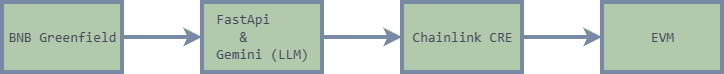
\includegraphics[width=0.9\linewidth]{architecture.png}
    \caption{DeRAG-Oracle System Architecture and End-to-End Data Flow.}
    \label{fig:architecture}
\end{figure}

\subsection{Decentralized Off-Chain Storage}
Raw enterprise files are uploaded to BNB Greenfield. This storage layer provides a decentralized solution designed for persistence and distributed access, allowing reference to source documents without cluttering the EVM state.

\subsection{FastAPI RAG Middleware}
Upon an oracle request, a FastAPI middleware intercepts the query. It fetches the target objects from BNB Greenfield and processes them through a RAG pipeline powered by the Google Gemini Flash model. The LLM is strictly prompted to extract and calculate two selected indicator metrics from the unstructured text: a Liquidity Ratio (used as a proxy for the financial condition) and an Attrition Rate (used to represent the human capital dimension).

\subsection{Chainlink CRE Consensus \& Smart Contract Settlement}
Non-deterministic LLM outputs pose a unique risk to blockchain state transitions. We utilize the Chainlink CRE to execute the middleware response across multiple independent oracle nodes. The consensus payload is then relayed to the BNB Smart Chain (BSC) Testnet. The receiving contract, \texttt{DeRAGReceiver.sol}, was compiled and verified via Remix IDE. Remix IDE served as the primary development environment to validate the Application Binary Interface (ABI) and ensure the \texttt{onReport()} function could accurately ingest the sub-400-byte string payload without triggering gas limit failures.

\section{Decentralized Consensus \& Security Model}
Integrating generative AI into deterministic blockchain environments requires strict consensus mechanisms to handle the inherent probabilistic nature of LLMs.

\subsection{Oracle Node Disagreement and Resolution}
When multiple oracle nodes process the same Greenfield document through the Gemini API, slight variations in text generation may occur. DeRAG implements a mode-based aggregation algorithm applied to the validated, normalized metric outputs. The consensus mechanism determines the accepted final value $V_{final}$ by requiring a supermajority (e.g., an illustrative threshold such as 2/3 of participating nodes) to agree on the core JSON schema and the extracted numerical metrics:
\begin{equation}
    V_{final} = \text{mode}(v_1, v_2, ..., v_n)
\end{equation}

\subsection{Failure to Reach Consensus}
If the network cannot reach a supermajority due to differing LLM interpretations resulting in widely divergent metric outputs, the consensus round fails. When no consensus is reached, the transaction is intentionally dropped, and no data is broadcast to the EVM. This fail-safe ensures that the smart contract state is never updated with contested or ambiguous data.

\subsection{Hallucination Detection and Source Grounding}
To detect unsupported LLM outputs, the DeRAG pipeline enforces strict source grounding. The extracted value is connected to evidence in the source document by requiring the LLM to output exact text citations alongside the calculated metrics. During consensus, nodes cross-validate these citations against the raw Greenfield file. If a node generates a hallucinated metric that does not match the source schema, its output is flagged as anomalous and discarded.

\subsection{Trust Assumptions and Correlated Failures}
A critical vulnerability in LLM-based oracles is correlated failure, which occurs when multiple oracle nodes make the exact same incorrect LLM inference. DeRAG's methodology assumes that prompt generation is constrained (e.g., using a Temperature of 0.0 to reduce sampling variability, though this does not mathematically guarantee deterministic underlying inference) and that the DON nodes operate independently. However, if the underlying LLM universally hallucinates the same incorrect metric, the DON will mistakenly reach consensus. Thus, the trust assumption relies heavily on the behavior of the underlying foundational model.

\section{Experimental Evaluation \& Benchmark}
To quantify the performance and economic viability of the DeRAG architecture, we conducted a systematic benchmark on the FastAPI middleware.

\subsection{Methodology and Statistical Significance}
A sample size of $N=30$ was selected as the benchmark sample size. While the Central Limit Theorem provides a general motivation for considering the sample mean's behavior under suitable conditions, this sample size serves as a methodological baseline to observe system latency rather than a universal guarantee of normality.

\subsection{Latency Evaluation}
While centralized RAG systems optimize strictly for speed, DeRAG introduces additional latency via decentralized consensus. Over the $N=30$ dataset, the system recorded a mean latency of:
\begin{equation}
    \mu = \frac{1}{30} \sum_{i=1}^{30} t_i = 6.882\text{ seconds}
\end{equation}
The 95th-percentile (P95) latency was recorded at 9.438 seconds, meaning approximately 95\% of observed requests had latency at or below this percentile during the benchmark executions.

\begin{figure}[H]
    \centering
    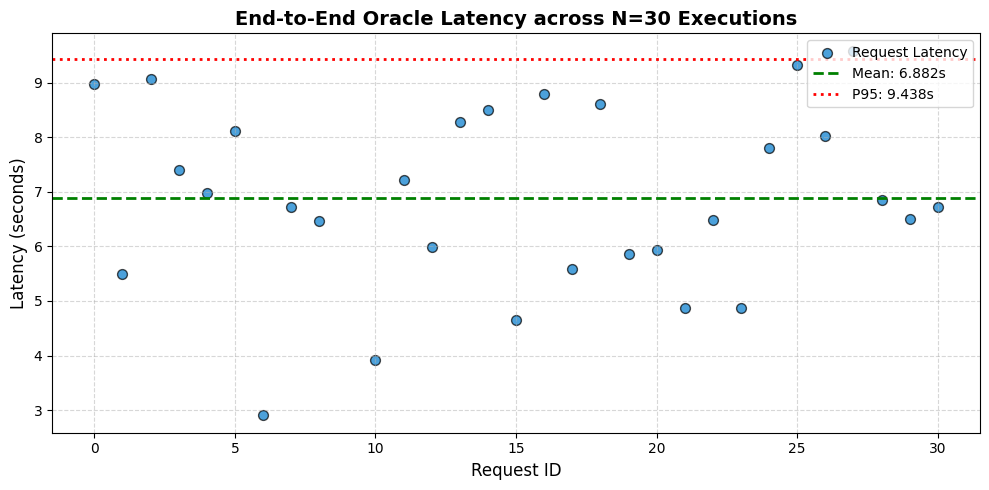
\includegraphics[width=0.8\textwidth]{latency_plot.png}
    \caption{Latency distribution across N=30 iterations, showing a P95 threshold of 9.438s.}
    \label{fig:latency}
\end{figure}

\begin{figure}[H]
    \centering
    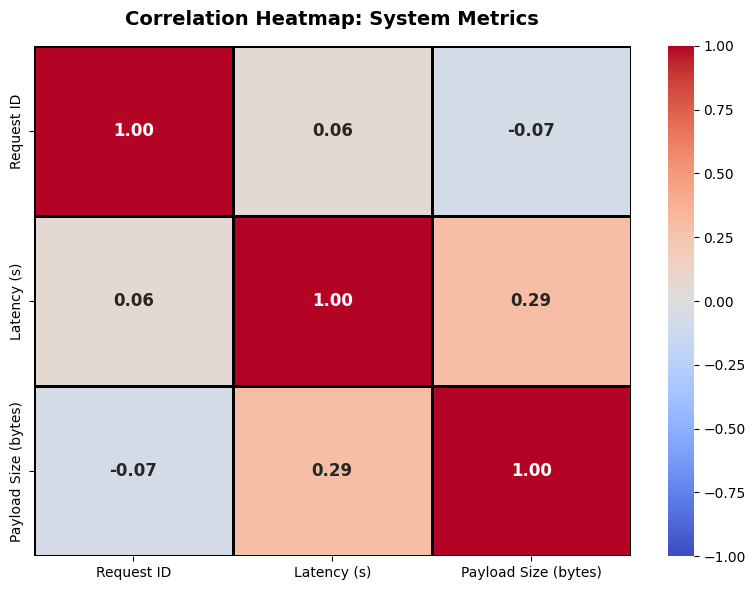
\includegraphics[width=0.75\textwidth]{correlation_heatmap.png}
    \caption{Correlation matrix of system metrics. The observed correlation of 0.06 indicates a negligible linear association between Request ID and Latency, providing no evidence of a strong temporal latency trend in the sampled executions.}
    \label{fig:heatmap}
\end{figure}

\subsection{Execution Stability \& Ground Truth}
The benchmark recorded a 100.0\% execution success rate (i.e., a 0.0\% observed execution failure rate). This metric exclusively measures system execution stability: the pipeline completed all 30 iterations without encountering dropped requests, crashes, or rate-limit HTTP errors, successfully returning a valid JSON schema in each instance. Because execution success does not inherently guarantee semantic correctness, the qualitative accuracy of the extractions was evaluated by manually cross-checking the source Greenfield files against the output JSON payloads to confirm that the model accurately extracted the specified metrics rather than generating unsupported values.

\begin{lstlisting}[language=json, caption=Example of the ultra-compact extracted risk payload.]
{
  "financial_risk_liquidity_ratio": 1.15,
  "human_capital_attrition_rate_pct": 12.4
}
\end{lstlisting}

\subsection{Payload Optimization and Expected On-Chain Efficiency}
The most significant metric captured was payload optimization. The average on-chain payload size was reduced to precisely 369.43 bytes. Assuming a raw enterprise JSON or PDF document size of roughly 50,000 bytes, the DeRAG architecture achieves a semantic data reduction of approximately 99.26\%. By distilling larger unstructured files into compact text representations, DeRAG is designed to significantly reduce the on-chain data payload, which is expected to yield corresponding qualitative improvements in gas efficiency for smart contract execution.

\section{Limitations}
While highly optimized, the architecture relies heavily on the context window limits of the underlying LLM; exceptionally large enterprise PDFs must be chunked before analysis. Second, utilizing premium LLMs across a multi-node DON introduces high API execution costs per transaction, which must be carefully weighed against the gas efficiency expected on-chain.

\section{Conclusion}
We have proposed DeRAG-Oracle, a decentralized architecture bridging unstructured enterprise data with Web3 networks. By combining BNB Greenfield, Google Gemini Flash, and Chainlink CRE, the system successfully shifts the computational burden of text parsing off-chain. Validated against an $N=30$ benchmark, the architecture delivers structured insights to the EVM with a 6.882s mean latency, a 0.0\% observed execution failure rate, and highly optimized 369.43-byte payloads, making advanced AI-driven smart contracts more practically deployable.

\begin{thebibliography}{9}
\bibitem{nakamoto}
S. Nakamoto, ``Bitcoin: A Peer-to-Peer Electronic Cash System,'' 2008. [Online]. Available: https://bitcoin.org/bitcoin.pdf

\bibitem{chainlink}
S. Ellis, A. Juels, and S. Nazarov, ``Chainlink: A Decentralized Oracle Network,'' 2017.

\bibitem{greenfield}
BNB Chain Community, ``BNB Greenfield: A Decentralized Data Storage Network and Economy,'' 2023.

\bibitem{rag}
P. Lewis et al., ``Retrieval-Augmented Generation for Knowledge-Intensive NLP Tasks,'' \textit{Advances in Neural Information Processing Systems}, vol. 33, pp. 9459-9474, 2020.
\end{thebibliography}

\end{document}